\documentclass[xcolor=table,usenames,dvipsnames]{beamer}

\usepackage[spanish]{babel}
\usepackage{courier}
\usepackage{xcolor}
\usepackage{mdframed}
\usepackage[utf8]{inputenc}
\usepackage{multicol,calc}
\usepackage{ragged2e} 
\usepackage{menukeys}
\usepackage{graphicx}
\usepackage{url}
\usepackage{amsmath, amsthm, amssymb}
\usepackage{setspace} %espaciado
\usepackage{etoolbox} %color bibliografía
\usepackage{wrapfig} %imagen alrededor texto
\usepackage{ajustes}



\title[Laboratorios SDR con GNU Radio (QT-2da Ed)]{
	Laboratorios SDR con GNU Radio}

\author[Ingeniería Electrónica]{Creación Colectiva\\
	\tiny 
	Bryan Estifen Garcia Zamora,
Juan David Cristancho Gaona,
Carlos Fernando Bustos Quevedo,
Carlos Mario Herrera Fernandez,
Esther Alexandra Ramos Arias,
Héctor Javier Vega Lozano,
Ferney Genaro Vasquez Sanabria,
Luis Mateo Cuervo Romero,
Julian Fernando Barreto Coronado,
Sergio Andres Dimas Gomez,
Leonardo Nicolas Solorzano Cruz,
Alex Isaac Urrea Mahecha,
Anderson Trullo Arias,
Pedro Yovan Munca Cadena\\
	\scriptsize
	Tutor\\ 
	\tiny
	Rodríguez Mújica Leonardo}

\institute[Universidad de Cundinamarca]{
	Facultad de Ingeniería\\
	Universidad de Cundinamarca}

\date{Diciembre 2021}

%-----------------------------------

\begin{document}
	
	%espaciado item
	\let\olditemize\itemize
	\def\itemize{\olditemize\itemsep=4pt }
	\footnotesize
	
	\begin{frame}
	\titlepage
\end{frame}
%-----------------------------------

\begin{frame}
\frametitle{Contenidos generales}
\tableofcontents[subsectionstyle=hide/hide, subsubsectionstyle=hide/hide]
\end{frame}
%-----------------------------------


%-----------------------------------

\section{LABORATORIOS CON SOFTWARE}
\begin{frame}

\pgfdeclareimage[width=\paperwidth,height=\paperheight]{bg}{imagenes/fondo_seccion}
\setbeamertemplate{background}{\pgfuseimage{bg}}

\definecolor{greenU}{RGB}{212,202,72}
\setbeamercolor{block body}{fg=Black,bg=greenU}
\begin{block}{}
\centering
\vspace{8mm}
\Large{LABORATORIOS CON SOFTWARE}
\vspace{8mm}
\end{block}
\end{frame}
%-----------------------

{
\begin{frame}
\frametitle{Parte I - Tabla de contenidos}
\begin{spacing}{1.5}
\tableofcontents[currentsection,sectionstyle=hide/hide,subsectionstyle=show/show/hide, subsubsectionstyle=hide]
\end{spacing}
\end{frame}
}

%///////////////////////////////////////////////////////////////
\subsection{Introducción a GNU Radio}

\begin{frame}{}

\pgfdeclareimage[width=\paperwidth,height=\paperheight]{bg}{imagenes/fondo_lab}
\setbeamertemplate{background}{\pgfuseimage{bg}}

\bfseries{\textrm{\Large \\Introducción a GNU Radio}}
\raggedright
\end{frame}



\begin{frame}
  
\pgfdeclareimage[width=\paperwidth,height=\paperheight]{bg}{imagenes/fondo3}
\setbeamertemplate{background}{\pgfuseimage{bg}}
  
  \frametitle{¿Qué es GNU Radio\index{GNU RADIO}?}

  
  Es una herramienta de desarrollo libre y abierta que provee bloques de procesamiento de señal para implementar sistemas de radio definido por software. Puede utilizarse con hardware de RF para crear radios definidos por
software o sin hardware para crear un ambiente de simulación. Es utilizada
extensivamente en ambientes académicos, aficionados y comerciales para dar
soporte a la investigación en comunicaciones inalámbricas y en sistemas de
radio en el mundo.
\end{frame}



\begin{frame}{Aplicaciones\index{Aplicaciones}}
  \begin{figure}[H]
  \centering
  \includegraphics[width=0.9\textwidth]{parte1/intro/pdf/intro.pdf}
  \end{figure}
  
  
\end{frame}



\begin{frame}{Instalación de GNU Radio en Linux}
{Para instalar GNU Radio se deben seguir los siguientes pasos:}
\begin{enumerate}[1.]
\item Ingresar a la ventana de órdenes (o terminal) del sistema de su equipo.
\item Estando conectado a internet, escriba dentro del terminal:

  \begin{block}{}
  \texttt{ sudo apt-get install gnuradio}
  \end{block}

\item Si su dispositivo tiene contrase\~na, debe ingresarla, al ser solicitada y oprimir \keys{\return}. 
\item Luego se deben aceptar los términos de la instalación oprimiendo la letra \keys{s} seguido de \keys{\return}. 
\item Una forma de verificar la correcta instalación es volviendo a ingresar la orden indicada en el punto 2, y si aparece un mensaje anunciando que GNU Radio ya está en su versión más reciente, su instalación fue correcta.
\end{enumerate}
\end{frame}
%----------------------------

\begin{frame}{Paquetes\index{Paquetes}}
Con el objetivo de clonar el repositorio y obtener los ejemplos de GNU Radio en nuestro ordenador se deben instalar los siguientes paquetes: 
  \begin{itemize}
  \item {\tt build-essential}

    Build essential es un paquete que contiene herramientas necesarias
    para la creación, compilación e instalación de programas.
  
  \item {\tt cmake}

  Es un sistema de construcción de código abierto multiplataforma. Se trata de
un conjunto de herramientas diseñadas para construir, testear y empaquetar
software. Se utiliza para controlar el proceso de compilación de software
utilizando una plataforma sencilla y unos archivos de configuración
independientes del compilador.

  \end{itemize}

\end{frame}
%-------------------------------

\begin{frame}{Paquetes}
  \begin{itemize}
  \item {\tt git}

    Este paquete contiene un sistema de control de versiones
distribuidas de código abierto desarrollado originalmente por Linux Torvalds
para apoyar el desarrollo del kernel de Linux.
    
	El control de versiones es un sistema que registra los cambios
realizados sobre un archivo o conjunto de archivos a lo largo del tiempo, de
modo que se puedan recuperar versiones específicas más adelante.
  
	\item {\tt libboost-all-dev} 
  
	Boost es un conjunto de bibliotecas para el lenguaje de programación
C++ que suministra un apoyo para tareas y estructuras como álgebra lineal,
generación de números pseudoaleatorios, procesamiento de imágenes, expresiones
regulares y pruebas unitarias. En el momento contiene 162 bibliotecas
individuales.
  
	\end{itemize}
\end{frame}

%++++++++++++++++++++

\begin{frame}{Paquetes\index{Paquetes}}
  \begin{itemize}
  \item {\tt libcppunit-dev}
  \begin{itemize}
    \item
    {Biblioteca de pruebas unitarias para C++.}
    \item
    {Una prueba unitaria es una forma de comprobar el correcto
funcionamiento de una unidad de código. Por ejemplo, en diseño
estructurado o en diseño funcional, una función o un procedimiento,
en diseño orientado a objetos una clase. Esto sirve para asegurar que
cada unidad funcione correcta y eficientemente por separado.}
    \end{itemize}
  \item {\tt doxygen}
  {Es una herramienta para generar documentación a partir de código fuente. Es un sistema de documentación para C++, C, Java, Python. Es necesario solo si se desea generar referencias a documentación externa de la que no tiene las fuentes.}
  \end{itemize}
\end{frame}

%+++++++++++++++++++

\begin{frame}{Instalación de paquetes}
\begin{enumerate}[1.]
\item La instalación de cada uno se los paquetes anteriormente mencionados se realiza colocando en la ventana de terminal, las siguientes órdenes:
\end{enumerate}

  \begin{block}{}
  \texttt{
  \ \ \ sudo apt-get install build-essential
    \begin{itemize}
      \item[] sudo apt-get install cmake
      \item[] sudo apt-get install git
      \item[] sudo apt-get install libboost-all-dev
      \item[] sudo apt-get install libcppunit-dev
      \item[] sudo apt-get install doxygen
    \end{itemize}}
  \end{block}


\end{frame}

%++++++++++++++++++++


\begin{frame}{Clonar repositorio\index{Clonar Repositorio}}
El código fuente de los ejemplos está almacenado en github, por lo tanto para clonar el repositorio se debe realizar lo siguiente:
\begin{itemize}
\item Abrir la ventana de órdenes o terminal.
\item Después se debe ingresar la siguiente orden para clonar el directorio git:

\begin{block}{}
  \texttt{
    git clone https://github.com/gnuradio/gr-tutorial}
  \end{block}

\item Una vez clonado el directorio, {\tt gr-tutorial}, en el PC empleado se deben ver exactamente los mismos archivos y carpetas que los del repositorio github.
\end{itemize}
\end{frame}

%+++++++++++++++++++

\begin{frame}{Instalación de módulos\index{Modulos}}
\begin{itemize}
\item Luego de haber clonado el repositorio, debemos buscar la carpeta \textbf{“gr-tutorial”} e ingresar a ella desde el terminal, para ello se digitan las siguientes órdenes:

  \begin{block}{}
  \texttt{
  \ \ \ ls
    \begin{itemize}
      \item[] cd gr-tutorial
    \end{itemize}}
  \end{block}

Es importante mencionar que al escribir la primera orden se podrán observar la diferentes carpetas que se encuentran en el dispositivo, por lo tanto \textbf{“gr-tutorial”} debe aparecer entre las opciones para poder cambiar de directorio. 
\end{itemize}
\end{frame}

%+++++++++++++++

\begin{frame}{Instalación de módulos\index{Modulos}}
\begin{itemize}
\item Estando dentro de la carpeta, desde la terminal, se deben escribir las siguientes órdenes, con la finalidad de instalar las soluciones o módulos:

  \begin{block}{}
  \texttt{
  \ \ \ mkdir build
    \begin{itemize}
      \item[] cd build
      \item[] cmake ..
      \item[] make -j8
      \item[] sudo make install
      \item[]sudo ldconfig
    \end{itemize}}
  \end{block}

\end{itemize}
\end{frame}

\begin{frame}{Resultado}
En el directorio {\tt examples} encontrará los tutoriales:
  \begin{block}{}
  \texttt{
    \begin{itemize}
      \item[] tutorial1
      \item[] tutorial2
      \item[] ...
      \item[] tutorial7
    \end{itemize}}
  \end{block}

Puede explorar los ejemplos de los desarrolladores de GNU Radio 
\end{frame}


%///////////////////////////////////////////////////////////////
\subsection{Lab1: Primeros pasos}
%*********************
\begin{frame}{}

\pgfdeclareimage[width=\paperwidth,height=\paperheight]{bg}{imagenes/fondo_lab}
\setbeamertemplate{background}{\pgfuseimage{bg}}

\bfseries{\textrm{\LARGE Lab1\\ \Large Primeros pasos}}
\raggedright
\end{frame}
%*********************

\begin{frame}{Primeros pasos}

\pgfdeclareimage[width=\paperwidth,height=\paperheight]{bg}{imagenes/fondo3}
\setbeamertemplate{background}{\pgfuseimage{bg}}

\begin{figure}[H]
\centering
\vspace{-3mm}
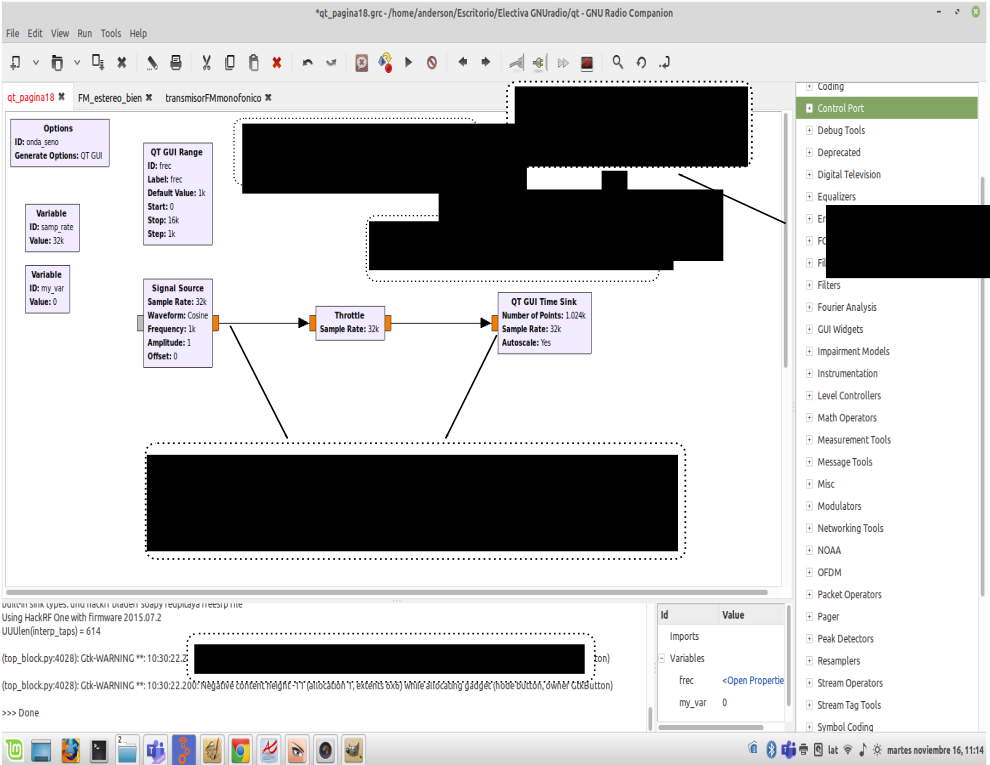
\includegraphics[width=0.9\textwidth]{parte1/lab1/pdf/lab1_1.pdf}
\end{figure}
\end{frame}
%-----------------------------------

\begin{frame}{Primeros pasos }
\begin{figure}[H]
\centering
\vspace{-3mm}
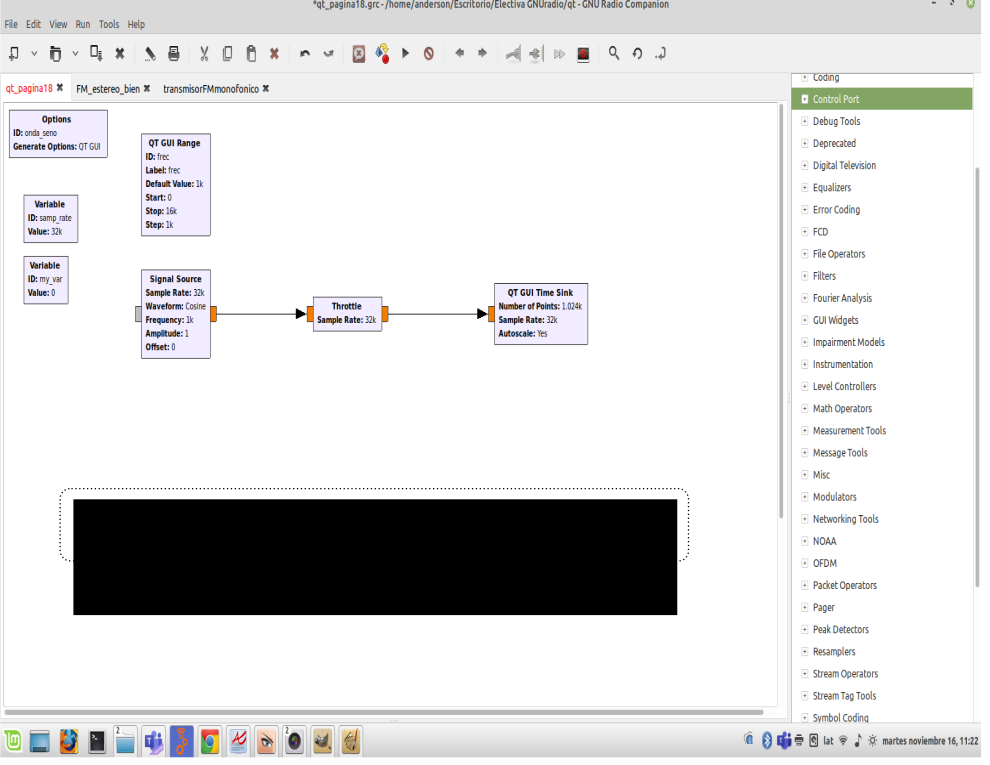
\includegraphics[width=0.9\textwidth]{parte1/lab1/pdf/lab1_2.pdf}
\end{figure}
\end{frame}
%-----------------------------------

\begin{frame}{Primeros pasos }
\begin{figure}[H]
\vspace{-3mm}
\centering
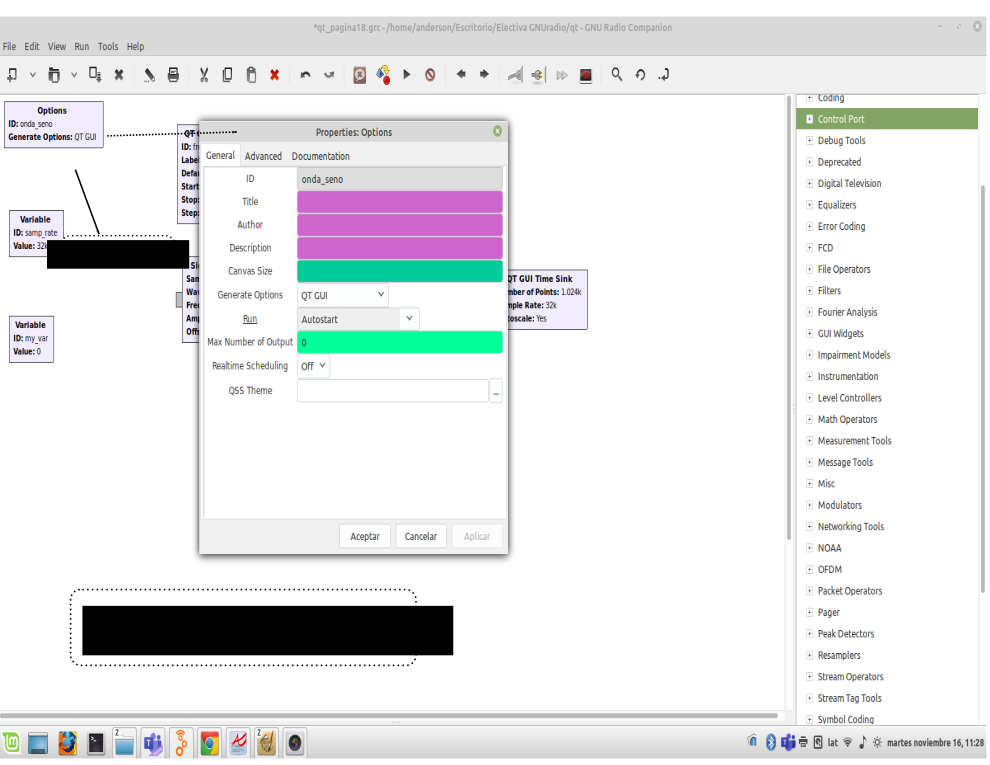
\includegraphics[width=0.9\textwidth]{parte1/lab1/pdf/lab1_3.pdf}
\end{figure}
\end{frame}
%-----------------------------------

\begin{frame}{Primeros pasos }
\begin{figure}[H]
\vspace{-3mm}
\centering
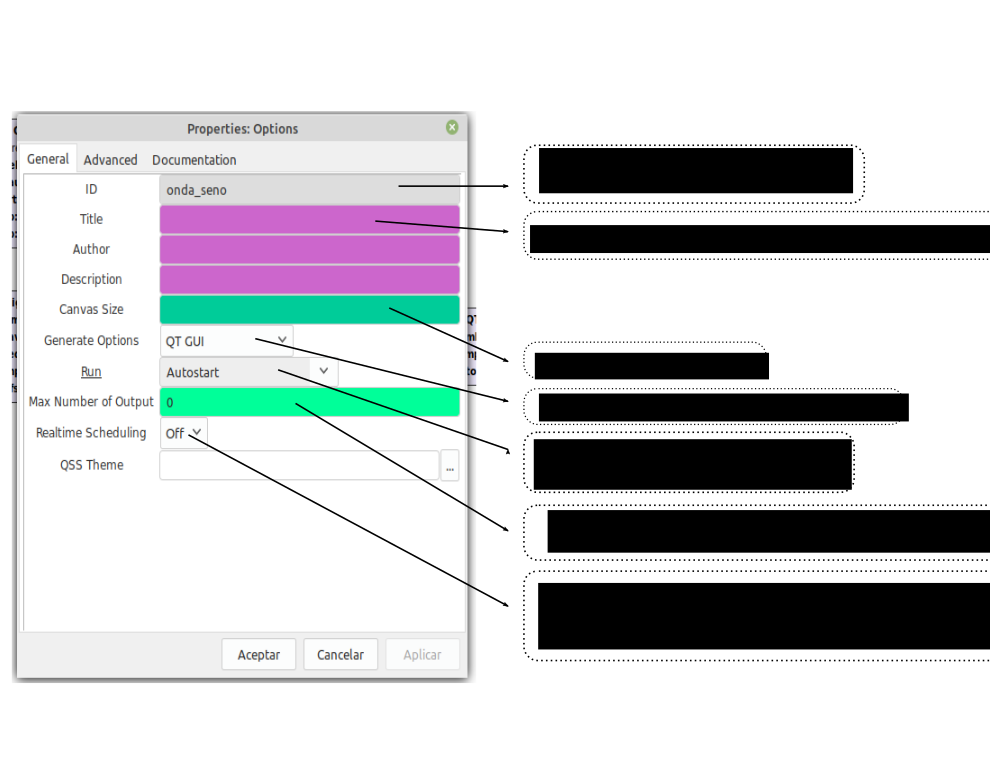
\includegraphics[width=0.9\textwidth]{parte1/lab1/pdf/lab1_4.pdf}
\end{figure}
\end{frame}
%-----------------------------------

\begin{frame}{Primeros pasos }
\begin{figure}[H]
\vspace{-2cm}
\centering
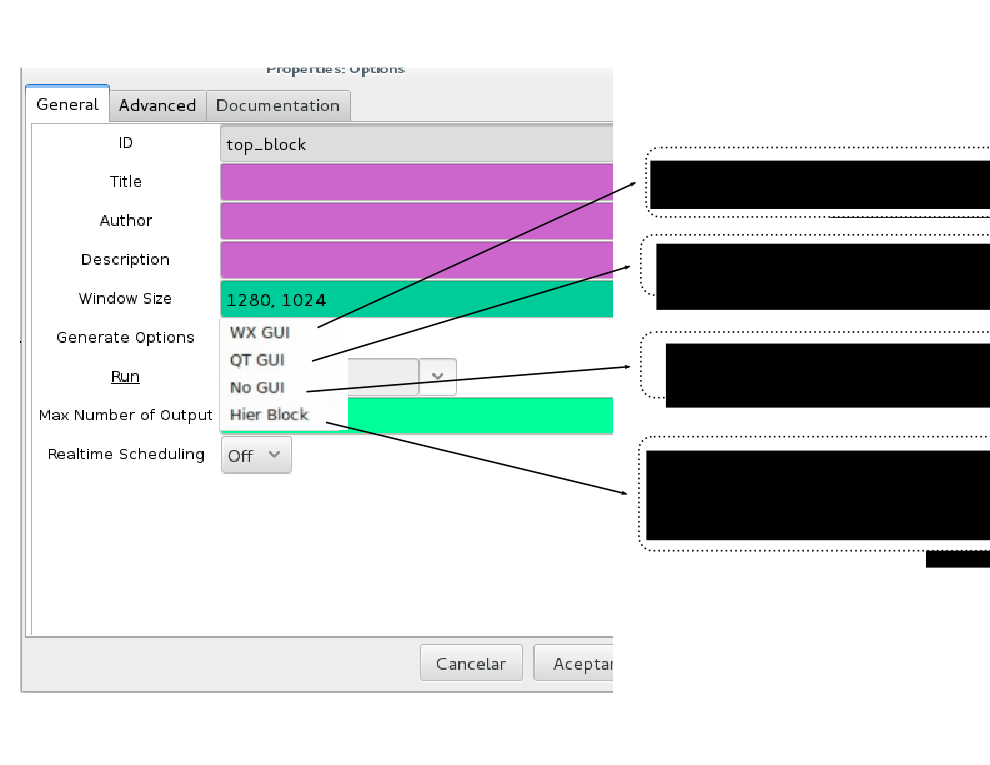
\includegraphics[width=1.1\textwidth]{parte1/lab1/pdf/lab1_5.pdf}
\end{figure}
\end{frame}
%-----------------------------------

\begin{frame}{Primeros pasos }
\begin{figure}[H]
\centering
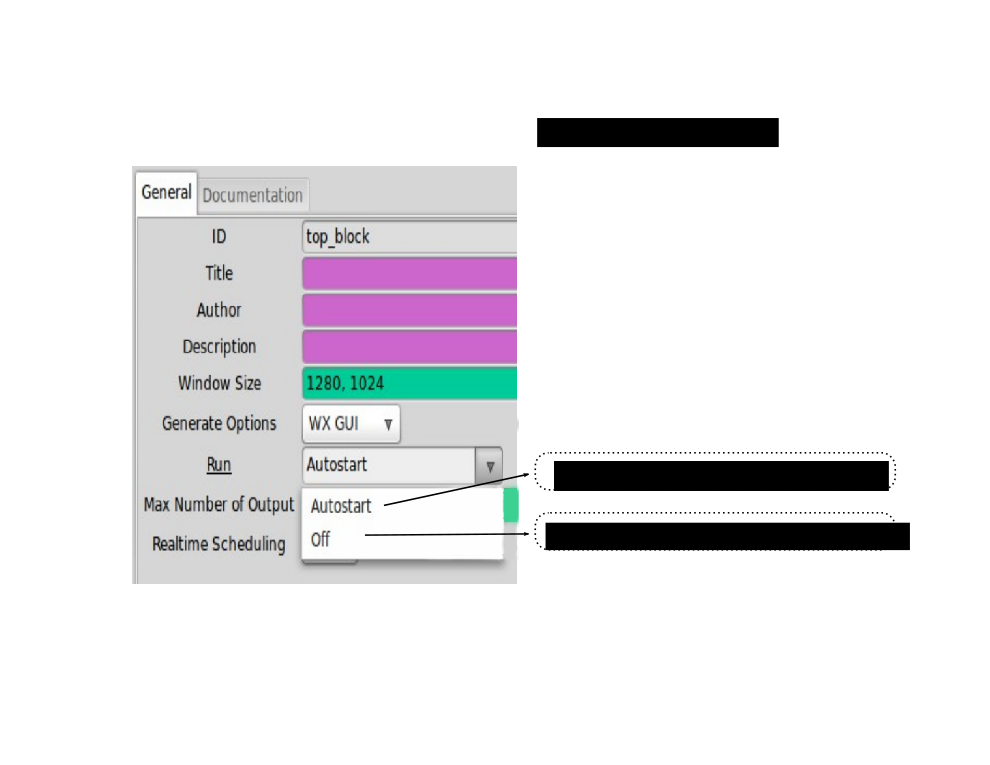
\includegraphics[width=.9\textwidth]{parte1/lab1/pdf/lab1_6.pdf}
\end{figure}
\end{frame}
%-----------------------------------

\begin{frame}{Primeros pasos }
\begin{figure}[H]
\centering
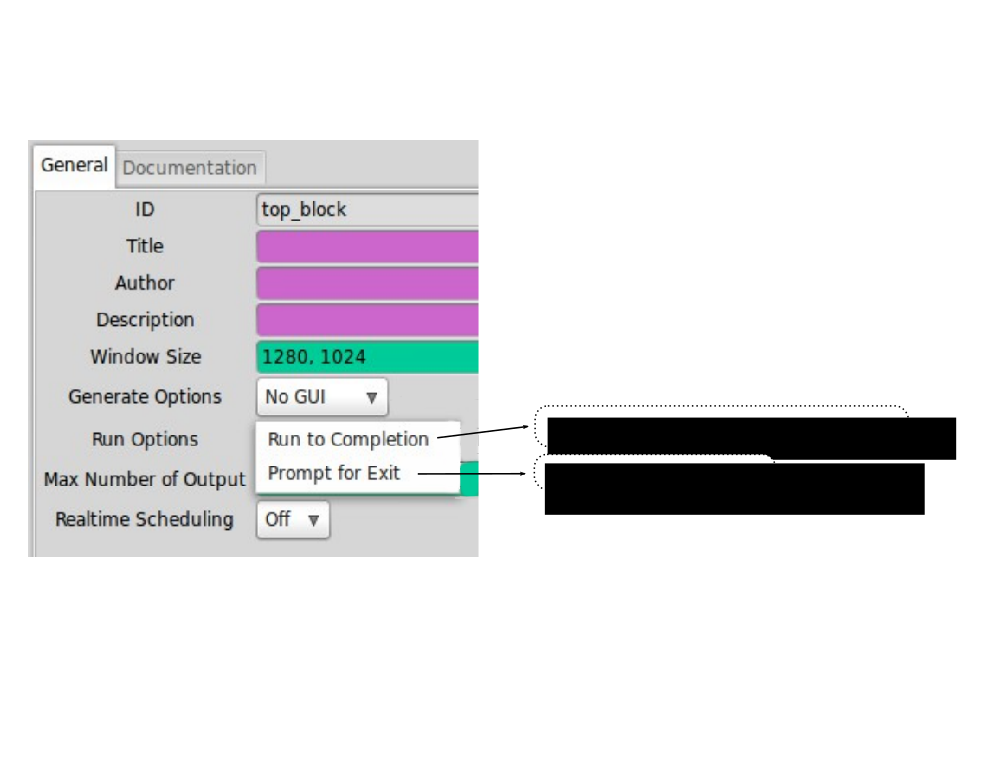
\includegraphics[width=\textwidth]{parte1/lab1/pdf/lab1_7.pdf}
\end{figure}
\end{frame}
%-----------------------------------

\begin{frame}{Primeros pasos }
\begin{figure}[H]
\vspace{-1cm}
\centering
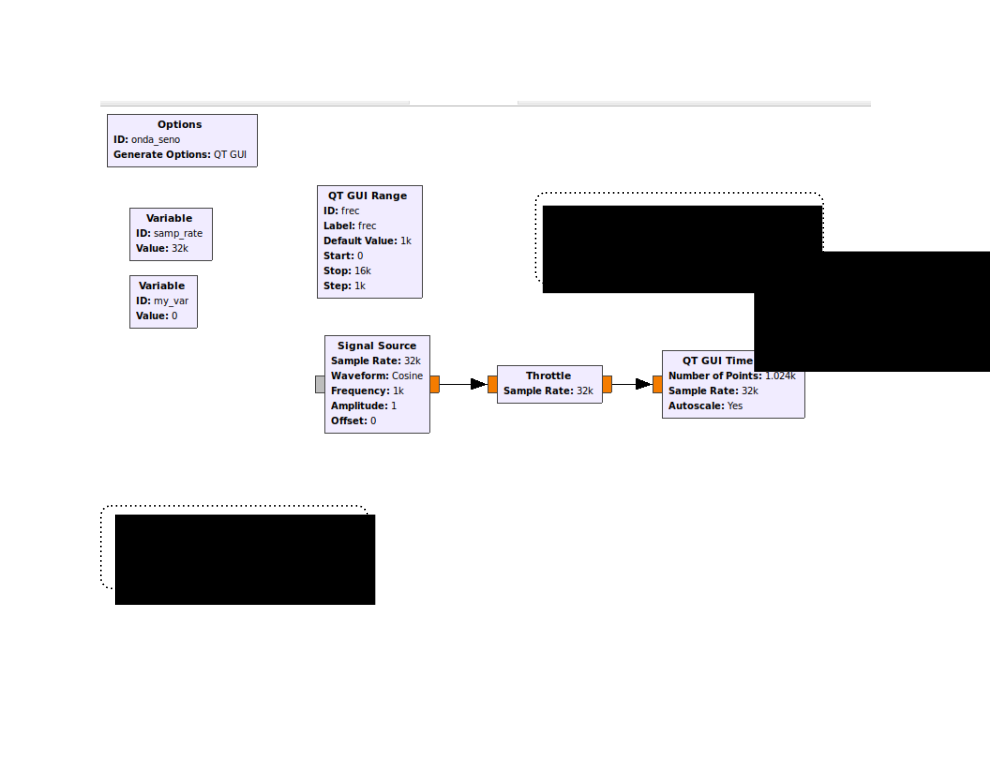
\includegraphics[width=\textwidth]{parte1/lab1/pdf/lab1_8.pdf}
\end{figure}
\end{frame}
%-----------------------------------

\begin{frame}{Primeros pasos }
\begin{figure}[H]
\vspace{-3mm}
\centering
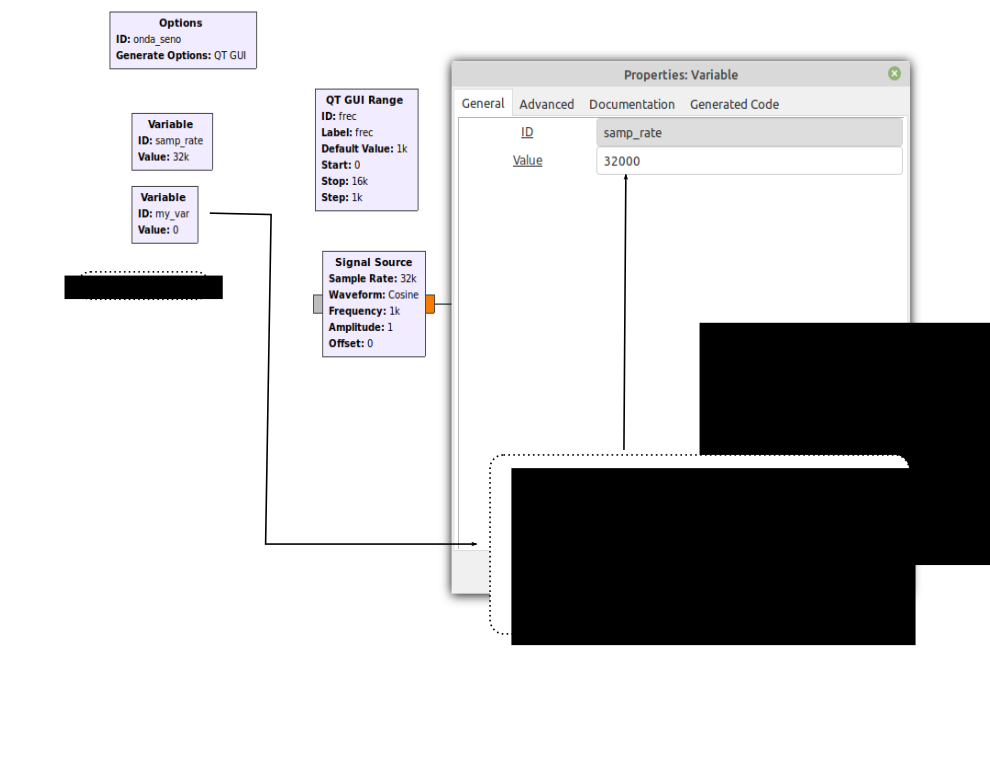
\includegraphics[width=0.85\textwidth]{parte1/lab1/pdf/lab1_9.pdf}
\end{figure}
\end{frame}
%-----------------------------------

\begin{frame}{Primeros pasos }
\begin{figure}[H]
\vspace{-3mm}
\centering
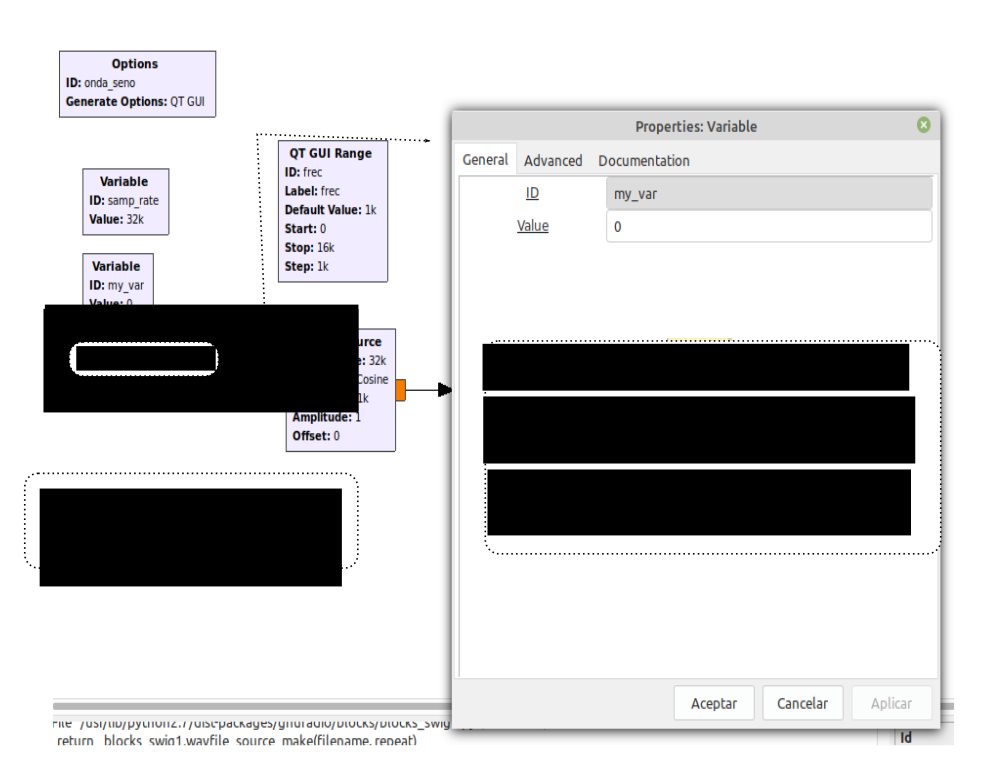
\includegraphics[width=.9\textwidth]{parte1/lab1/pdf/lab1_10.pdf}
\end{figure}
\end{frame}
%-----------------------------------

\begin{frame}{Primeros pasos }
\begin{figure}[H]
\vspace{-3mm}
\centering
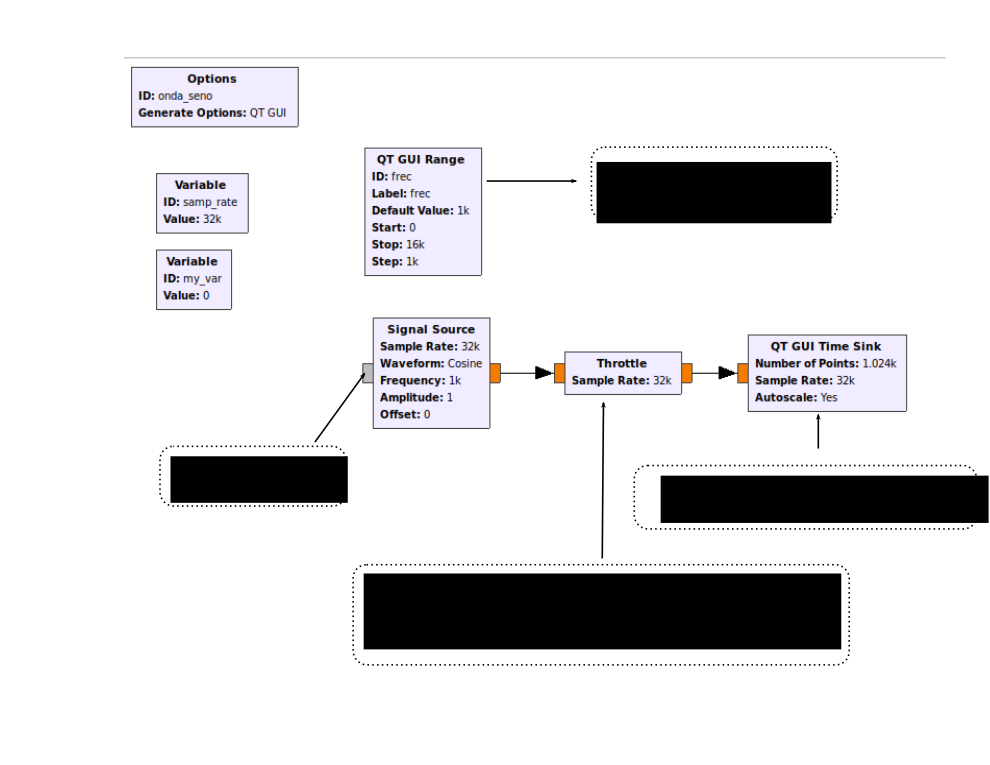
\includegraphics[width=\textwidth]{parte1/lab1/pdf/lab1_11.pdf}
\end{figure}
\end{frame}
%-----------------------------------

\begin{frame}{Primeros pasos }
\begin{figure}[H]
\vspace{-3mm}
\centering
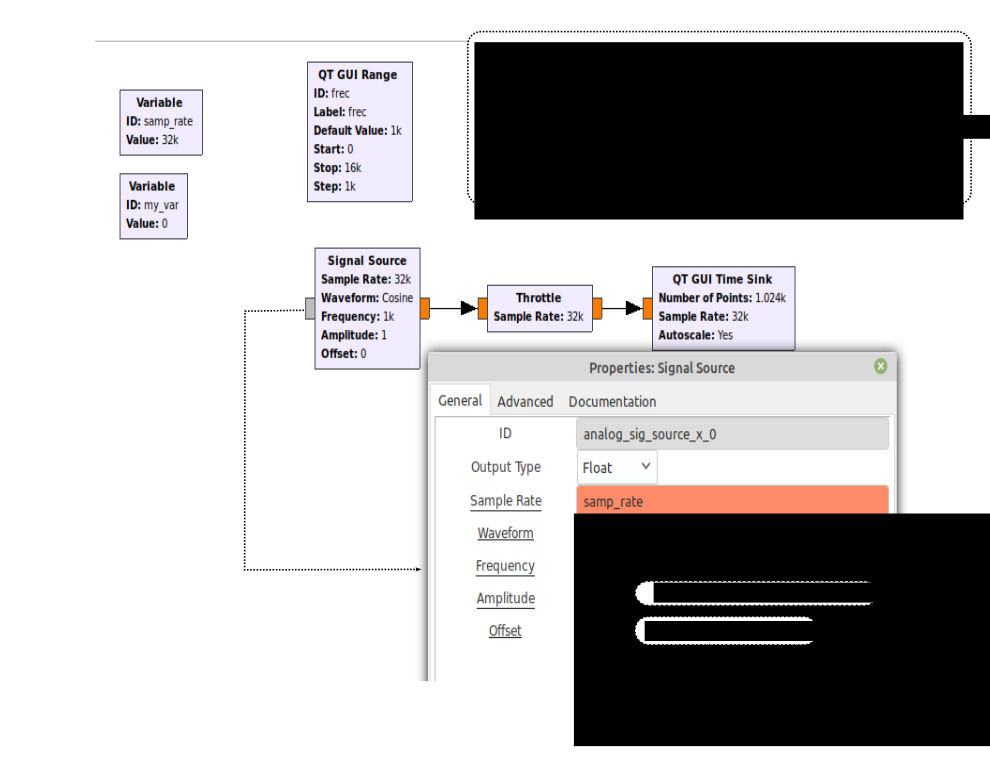
\includegraphics[width=.85\textwidth]{parte1/lab1/pdf/lab1_12.pdf}
\end{figure}
\end{frame}
%-----------------------------------

\begin{frame}{Primeros pasos }
\begin{figure}[H]
\vspace{-3mm}
\centering
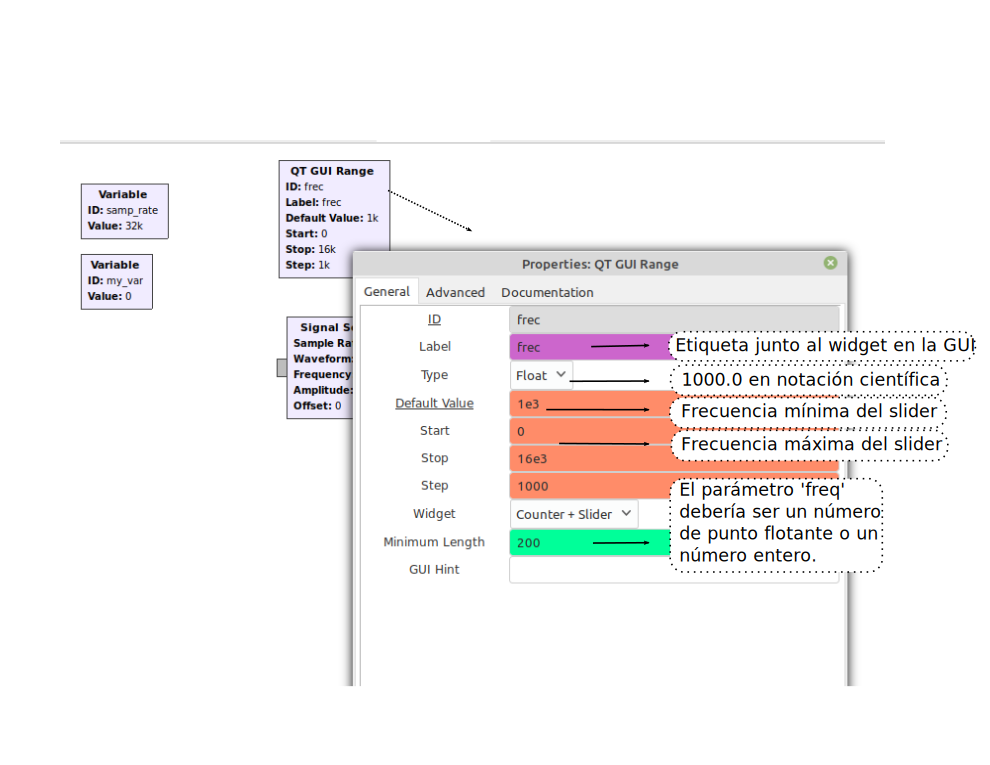
\includegraphics[width=\textwidth]{parte1/lab1/pdf/lab1_13.pdf}
\end{figure}
\end{frame}
%-----------------------------------

\begin{frame}{Primeros pasos }
\begin{figure}[H]
\vspace{-1cm}
\centering
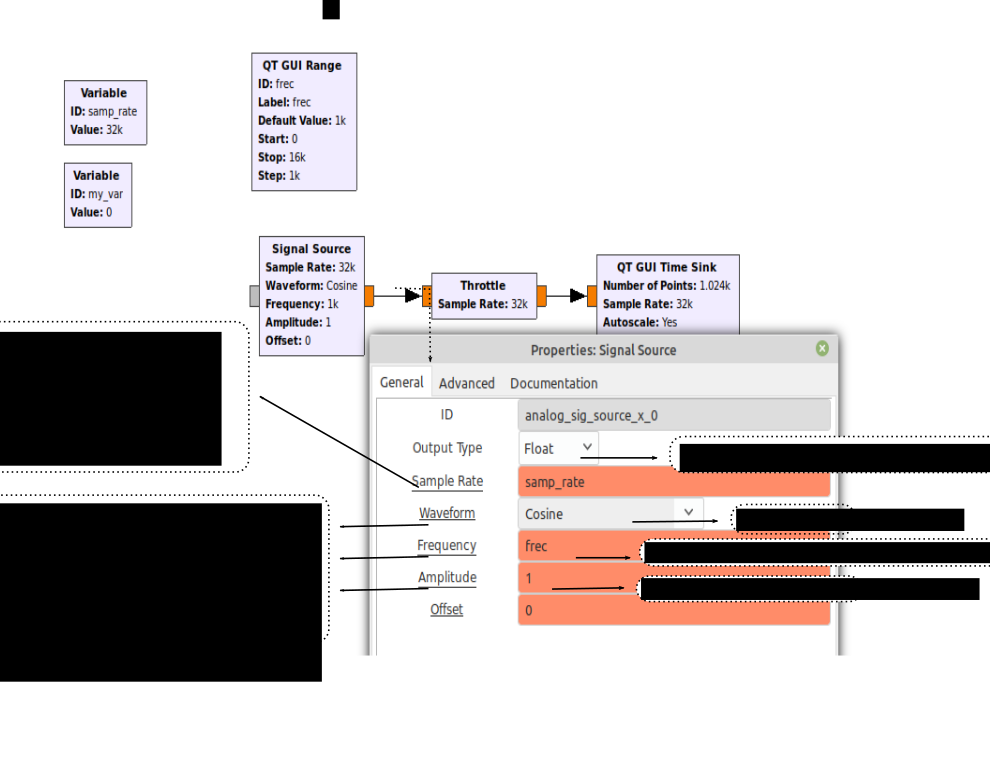
\includegraphics[width=1.05\textwidth]{parte1/lab1/pdf/lab1_14.pdf}
\end{figure}
\end{frame}
%-----------------------------------

\begin{frame}{Primeros pasos }
\begin{figure}[H]
\vspace{-3mm}
\centering
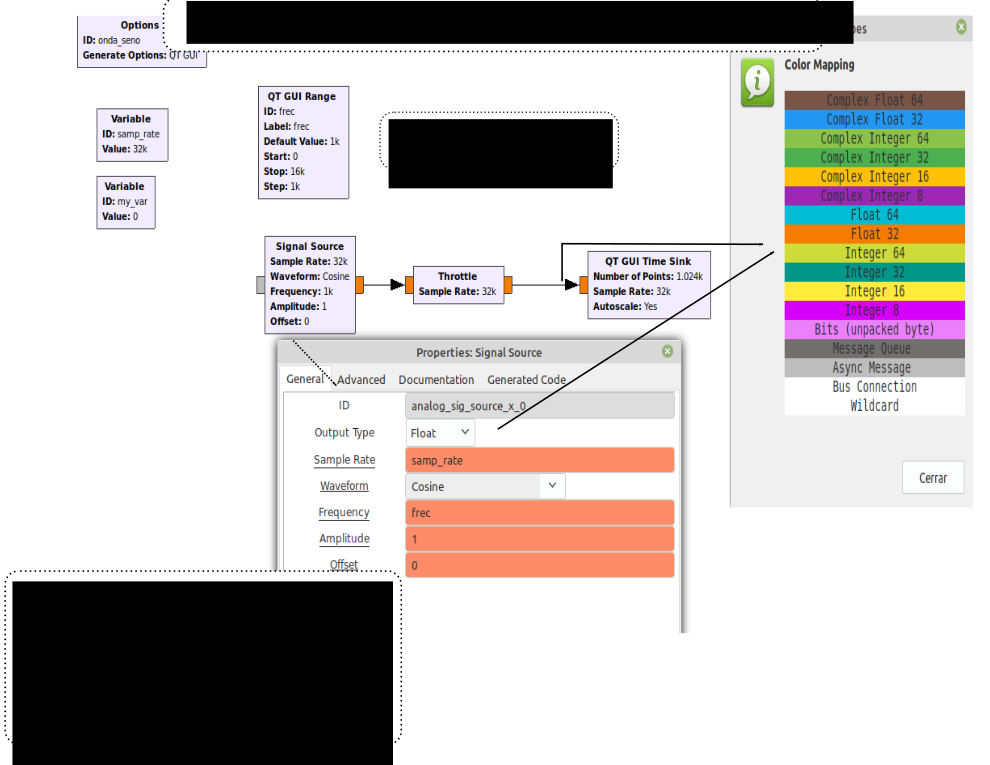
\includegraphics[width=.80\textwidth]{parte1/lab1/pdf/lab1_15.pdf}
\end{figure}
\end{frame}
%-----------------------------------

\begin{frame}{Primeros pasos }
\begin{figure}[H]
\centering
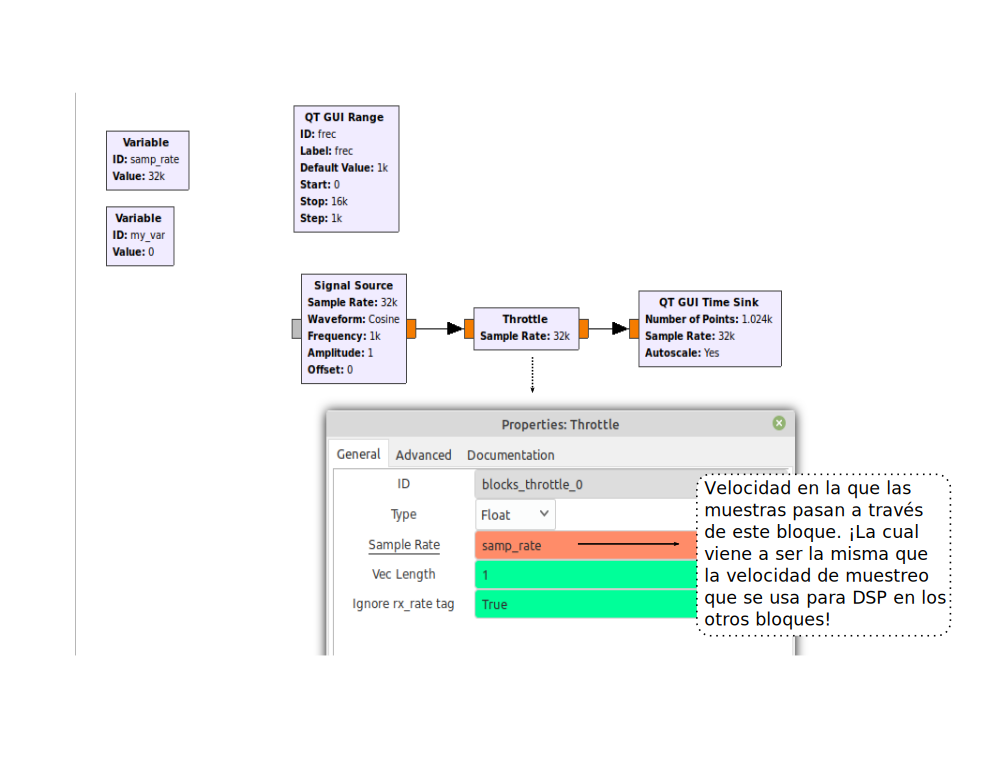
\includegraphics[width=\textwidth]{parte1/lab1/pdf/lab1_16.pdf}
\end{figure}
\end{frame}
%-----------------------------------

\begin{frame}{Primeros pasos }
\begin{figure}[H]
\vspace{-3mm}
\centering
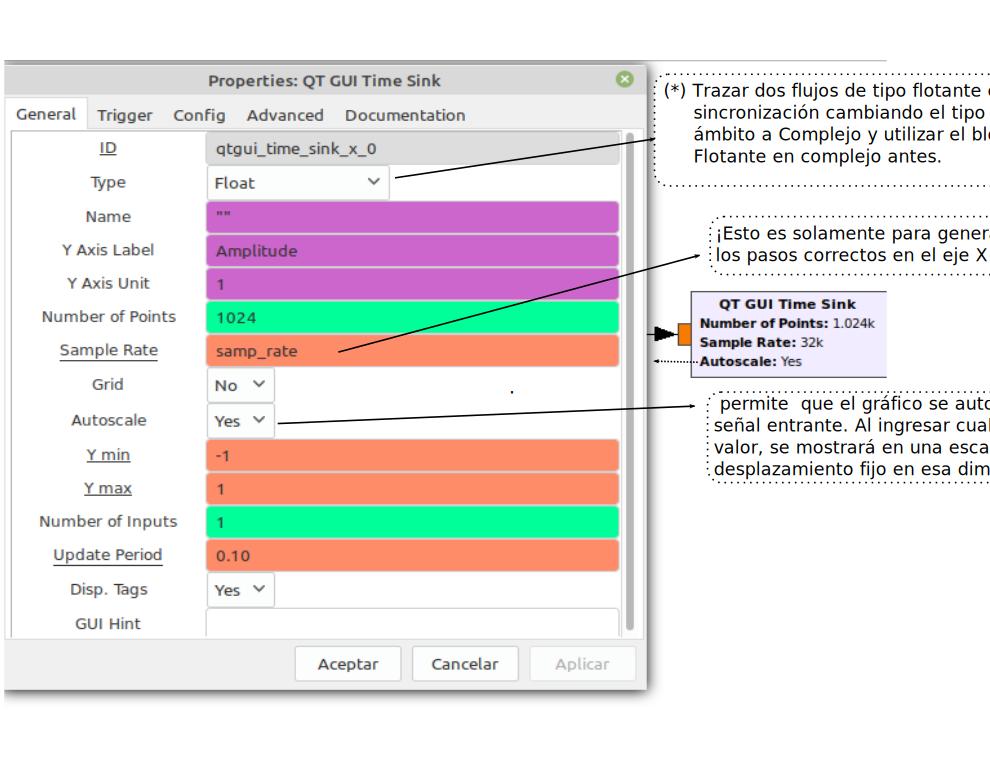
\includegraphics[width=.85\textwidth]{parte1/lab1/pdf/lab1_17.pdf}
\end{figure}
\end{frame}
%-----------------------------------

\begin{frame}{Primeros pasos }
\begin{figure}[H]
\centering
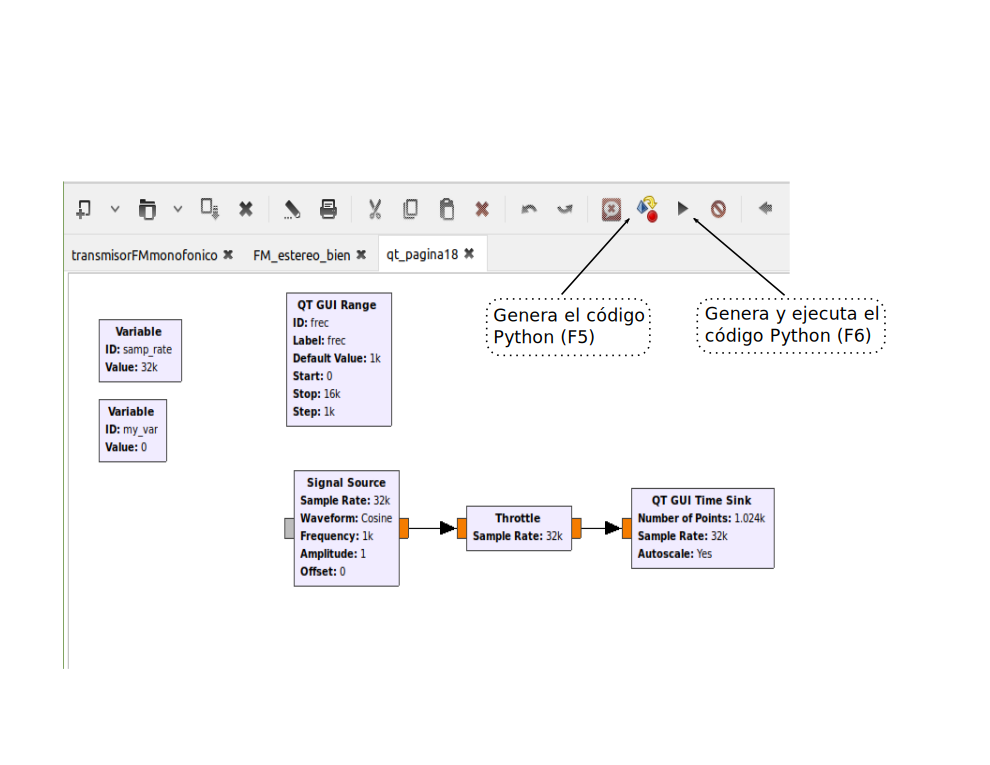
\includegraphics[width=\textwidth]{parte1/lab1/pdf/lab1_18.pdf}
\end{figure}
\end{frame}
%-----------------------------------

\begin{frame}{Primeros pasos }
Programa en Python generado por GRC
\begin{figure}[H]
\centering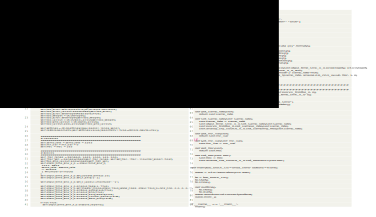
\includegraphics[width=0.95\textwidth]{parte1/lab1/pdf/lab1_18a.pdf}
\end{figure}
\end{frame}
%-----------------------------------

\begin{frame}{Primeros pasos }
\begin{figure}[H]
\centering
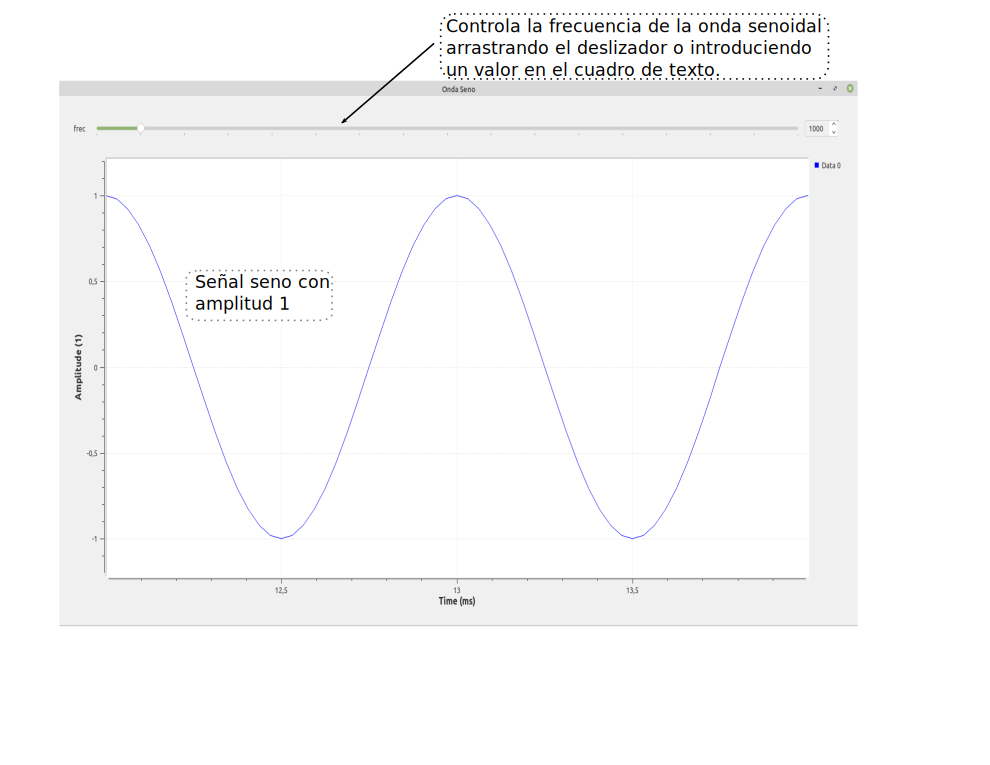
\includegraphics[width=\textwidth, height=0.55\textwidth]{parte1/lab1/pdf/lab1_19.pdf}
\end{figure}
\end{frame}
%-----------------------------------

\begin{frame}{Primeros pasos }
\begin{figure}[H]
\centering
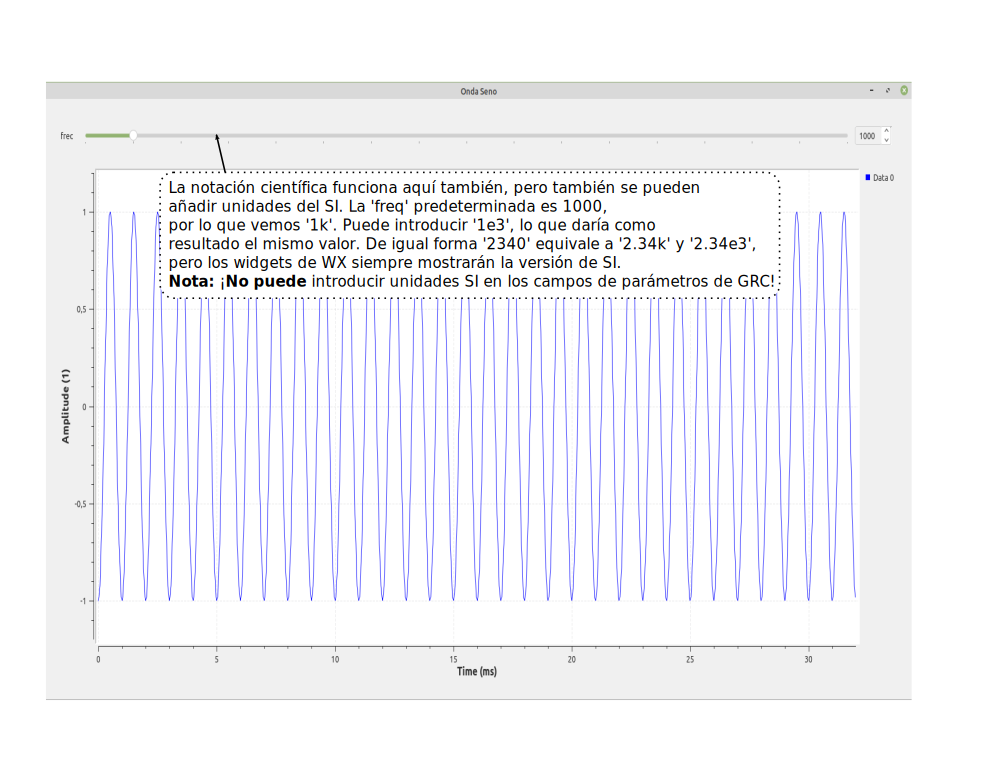
\includegraphics[width=\textwidth, height=0.55\textwidth]{parte1/lab1/pdf/lab1_20.pdf}
\end{figure}
\end{frame}
%-----------------------------------

\begin{frame}{Primeros pasos }
\begin{figure}[H]
\centering
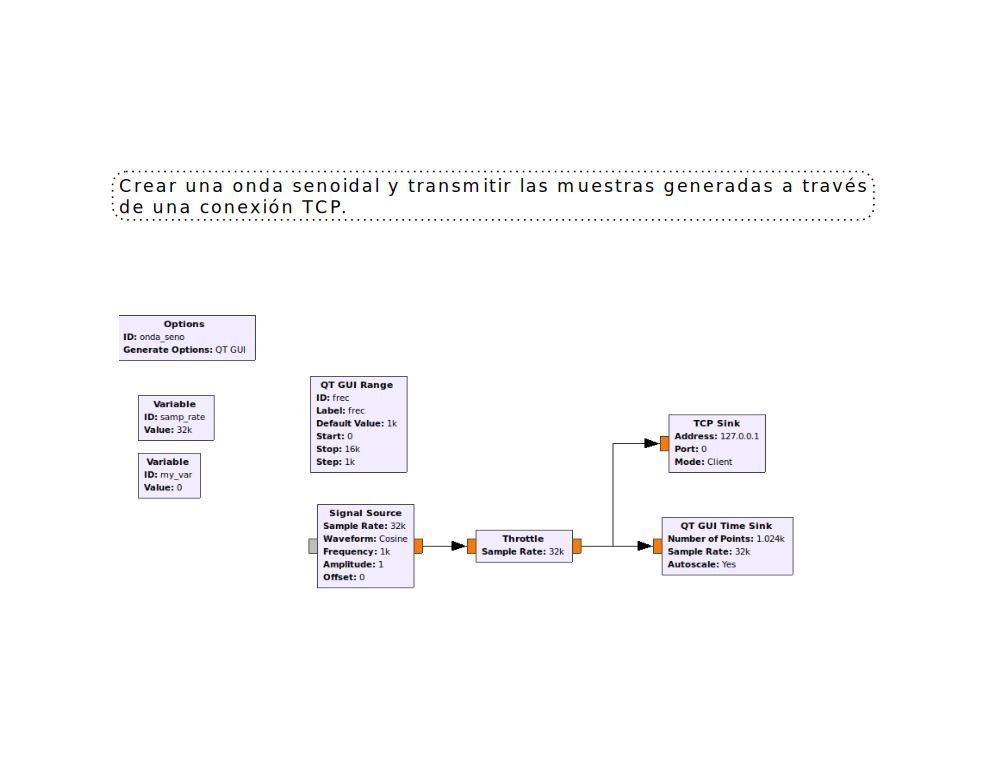
\includegraphics[width=\textwidth]{parte1/lab1/pdf/lab1_21.pdf}
\end{figure}
\end{frame}
%-----------------------------------

\begin{frame}{Primeros pasos }
\begin{figure}[H]
\centering
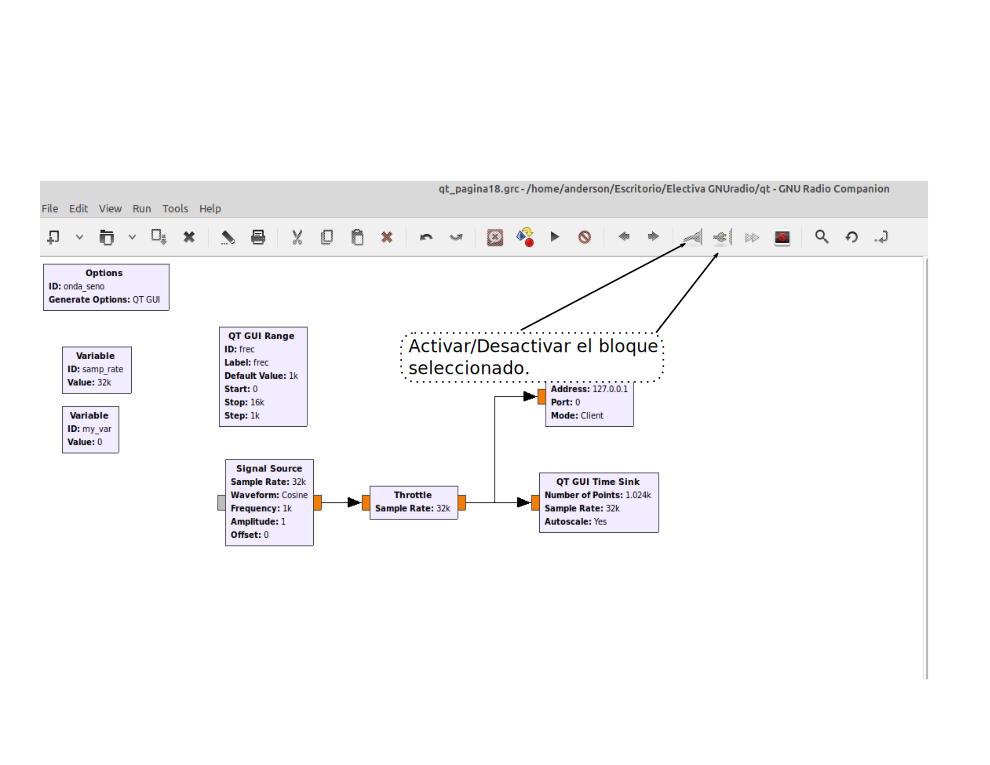
\includegraphics[width=\textwidth]{parte1/lab1/pdf/lab1_22.pdf}
\end{figure}
\end{frame}
%-----------------------------------

\begin{frame}{Primeros pasos }
\begin{figure}[H]
\centering
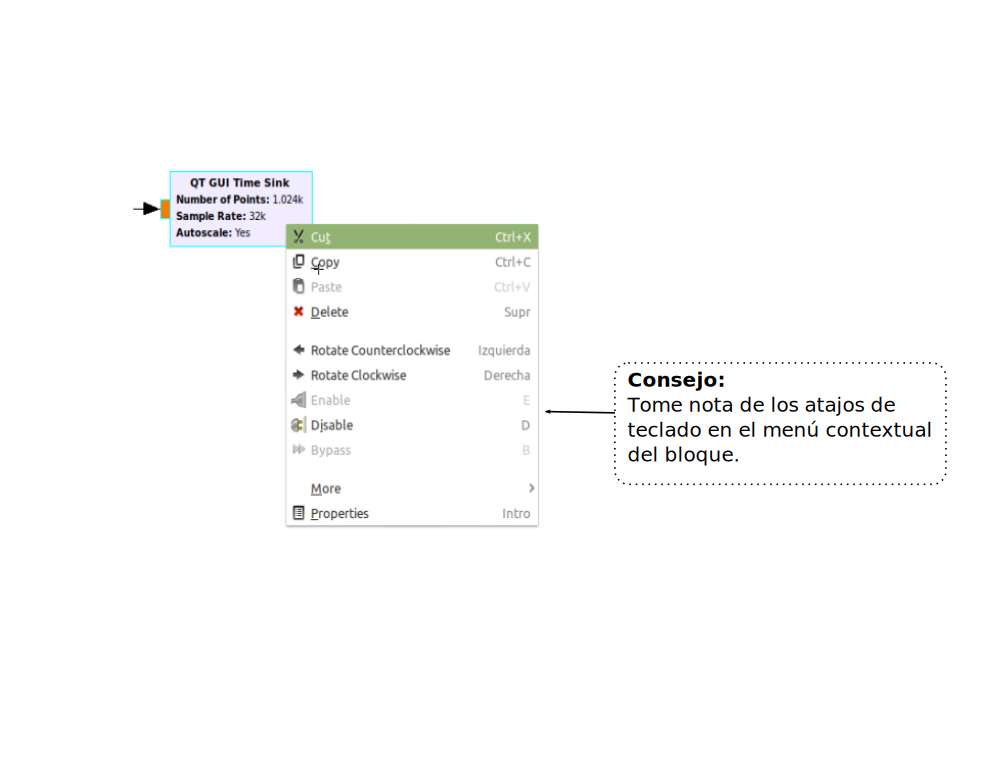
\includegraphics[width=\textwidth, height=0.6\textwidth]{parte1/lab1/pdf/lab1_23.pdf}
\end{figure}
\end{frame}
%-----------------------------------

\begin{frame}{Primeros pasos }
\begin{figure}[H]
\centering
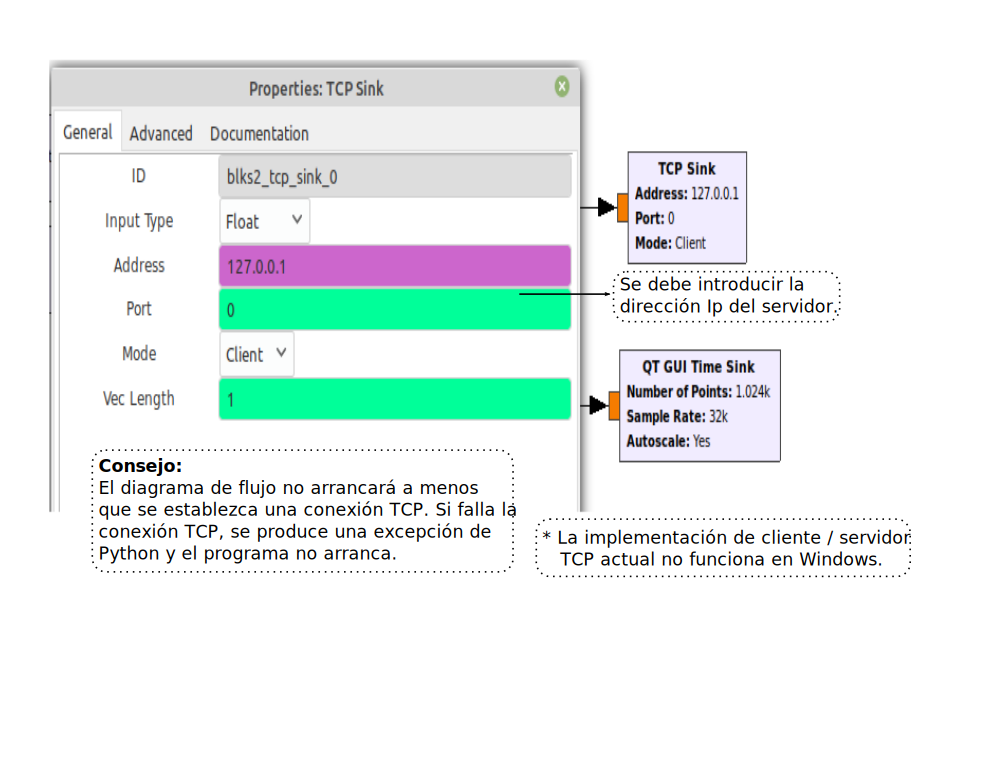
\includegraphics[width=\textwidth]{parte1/lab1/pdf/lab1_24.pdf}
\end{figure}
\end{frame}
%-----------------------------------

\begin{frame}{Primeros pasos }
\begin{figure}[H]
\centering
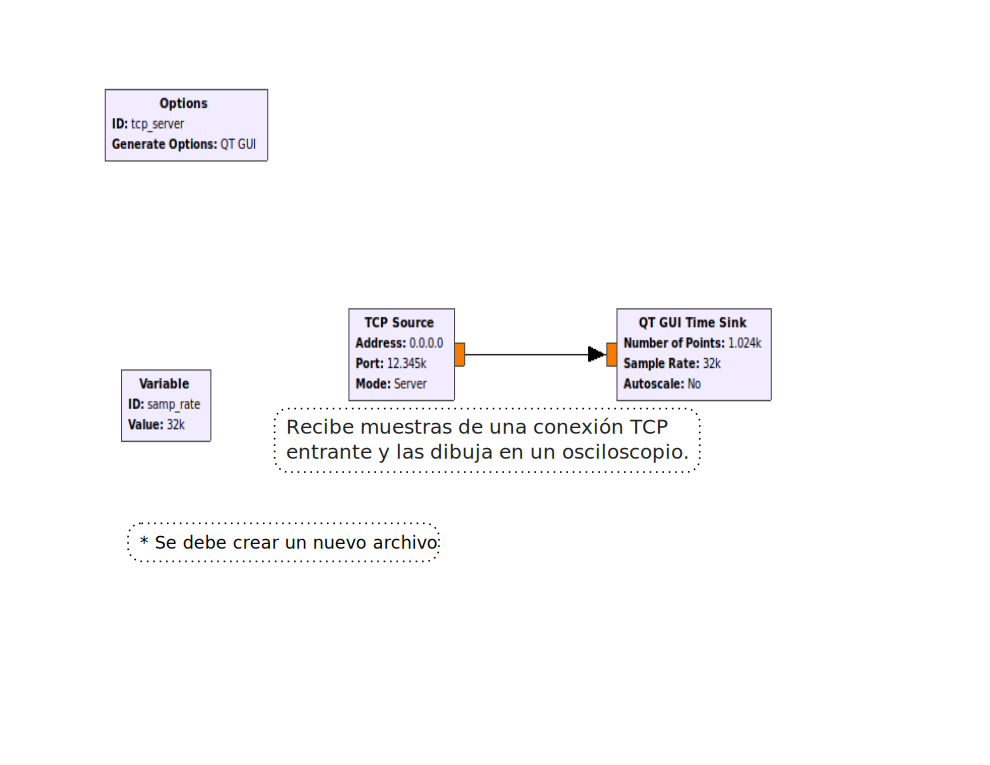
\includegraphics[width=\textwidth]{parte1/lab1/pdf/lab1_25.pdf}
\end{figure}
\end{frame}
%-----------------------------------

\begin{frame}{Primeros pasos }
\begin{figure}[H]
\centering
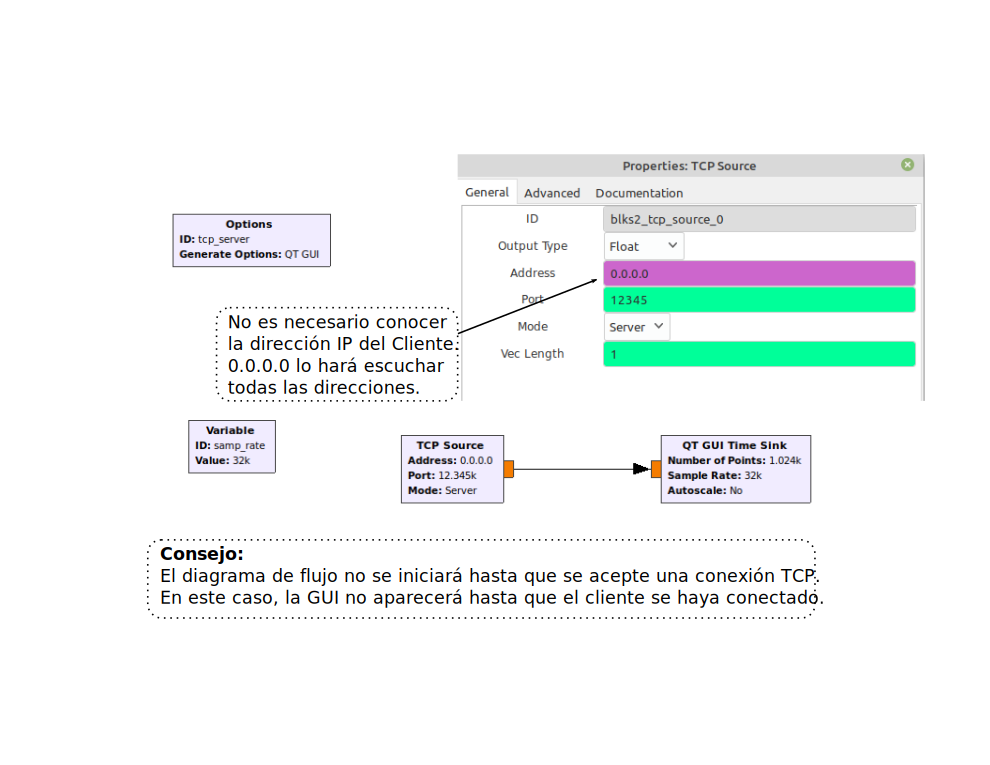
\includegraphics[width=\textwidth]{parte1/lab1/pdf/lab1_26.pdf}
\end{figure}
\end{frame}
%-----------------------------------

\begin{frame}{Primeros pasos }
\begin{figure}[H]
\centering
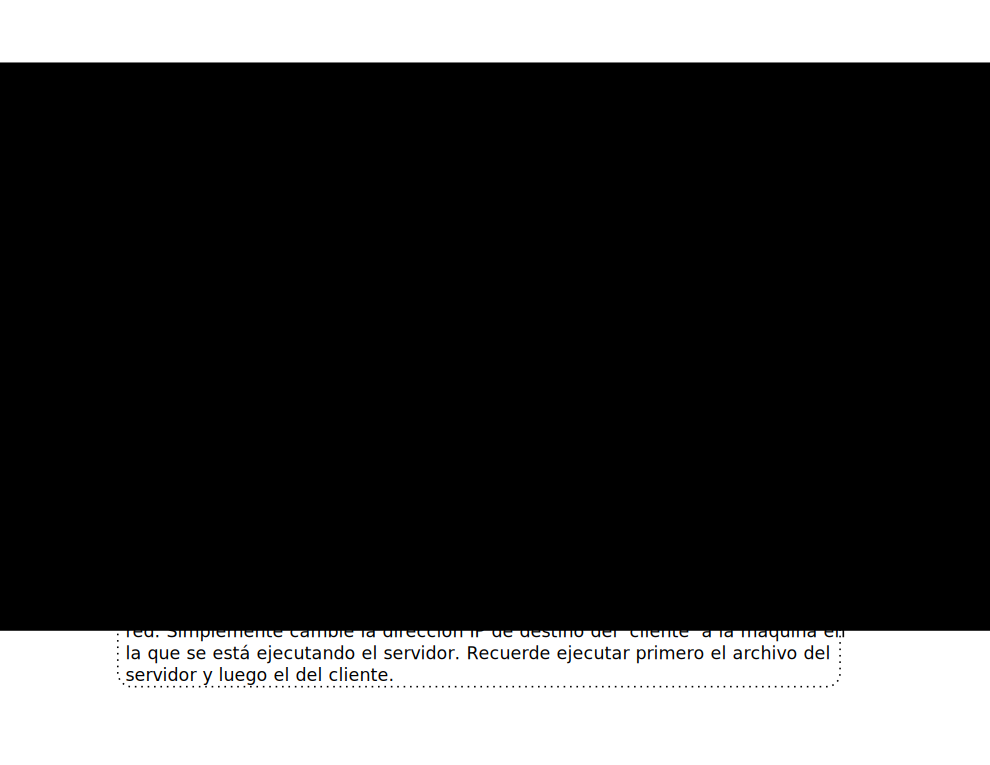
\includegraphics[width=\textwidth, height=0.55\textwidth]{parte1/lab1/pdf/lab1_27.pdf}
\end{figure}
\end{frame}
%-----------------------------------

\subsubsection{Actividad 1_lab1}
\begin{frame}

\pgfdeclareimage[width=\paperwidth,height=\paperheight]{bg}{imagenes/fondo_seccion}
\setbeamertemplate{background}{\pgfuseimage{bg}}

\definecolor{greenU}{RGB}{212,202,72}
\setbeamercolor{block body}{fg=Black,bg=greenU}
\begin{block}{}
	\centering
	%\vspace{1mm}
	\Large{\textit{Actividades}}
	%\vspace{1mm}
\end{block}
\end{frame}

\begin{frame}

\pgfdeclareimage[width=\paperwidth,height=\paperheight]{bg}{imagenes/fondo3}
\setbeamertemplate{background}{\pgfuseimage{bg}}

\frametitle{\underline{\textbf{Transmisión de señales por multiplexación}}}

En esta actividad usted debe transmitir 3 señales periódicas por medio del TCP (Protocolo de 	Control de Transmisión) desde el cliente, mediante el proceso de multiplexación de señales, al 	servidor, que se encargará de demultiplexar la señal recibida y mostrar las 3 que fueron  	transmitidas en el Scope Sink.\vspace{2mm}

Es importante saber que:
\begin{enumerate}[1.]
\item {La multiplexación es el proceso mediante el cual diferentes mensajes de información (Señales) se combinan en una única señal con el fin de trasmitirla. }\\

\item {La demultiplexación es el proceso mediante el cual la señal multiplexada recibida se divide en cada una de las señales que la generaron.}\\
\end{enumerate}
\end{frame}

%-----------------------------------

\begin{frame}

\pgfdeclareimage[width=\paperwidth,height=\paperheight]{bg}{imagenes/fondo3}
\setbeamertemplate{background}{\pgfuseimage{bg}}

\frametitle{\underline{\textbf{Pistas para la actividad}}}

Las pistas son:
\begin{enumerate}[1.]
	\item {Modo cliente: Bloques y conexiones de los primeros pasos. (WX GUI Slider, Signal Source, TCP Sink, Scope Sink, Throttle, Stream Mux, Variable)}
	
	\item {Modo servidor:  Bloques y conexiones de los primeros pasos. (TCP Source, Scope Sink, Stream to Streams)}
	\item {Multiplexación: Bloque Stream Mux. En el parámetro Lengths se debe agregar el número de ítems de cada señal, en forma de lista. Para la actividad las señales cuentan con un solo ítem. 
	Como ejemplo de lo anterior tenemos que: }
\begin{itemize}
	\item 2 señales = 1,1    
	\item 3 señales = 1,1,1 
	\item 4 señales = 1,1,1,1
\end{itemize}
	\item {Demultiplexación: Bloque Stream to Streams.}
    \item { El tipo de dato en todos los bloques debe ser el mismo. (float)}
	\item {Habilitar las entradas o salidas suficientes para los bloques.}
\end{enumerate}
\end{frame}

%-----------------------------------

%\begin{frame}{Actividad de los Primeros pasos }
%\begin{figure}[H]
%\centering
%\vspace{-3mm}
%\includegraphics[width=0.9\textwidth]{parte1/lab1/Actividades/pdf/prueba.pdf}
%\end{figure}
%\end{frame}
%-----------------------------------

\subsubsection{Actividad2}


\begin{frame}
	\frametitle{\underline{\textbf{Modificación de las variables de una señal periódica}}}
	
	Aprender a variar los componentes básicos de una señal periódica (amplitud, frecuencia, fase y nivel DC) en GNU Radio.\vspace{2mm}
	
	Es importante saber que:
	
	\begin{enumerate}[1.]
		\item{La forma más simple de representar una señal periódica es una senoidal como se presenta matemáticamente a continuación}\\
		
		$$x(t)=A\sin(2 \pi f + \phi) + K$$\\
		
		En donde:\\
		
		\item{Amplitud ($A$): Es el valor máximo que toma la señal, es decir, la distancia entre el punto máximo de la señal y cero, este punto puede ser tanto positivo como negativo.}\\
		
		\item{Frecuencia ($f$): Es el número de ciclos que realiza la señal por unidad de tiempo, esta medida está dada en Hertz (Hz), que equivale a un ciclo por segundo, lo que significa que 80 Hz son 80 ciclos por cada segundo que transcurre.}\\
		
	\end{enumerate}
\end{frame}


\begin{frame}
	\frametitle{\underline{\textbf{Modificación de las variables de una señal periódica}}}
	\begin{enumerate}[1.]
		
		\item{La fase ($\phi$): Indica la magnitud de una de variación ciclíca, siendo la fracción del período que transcurre desde el instante tomado al estado hasta la referencia, es decir el desplazamiento que tiene una señal en grados con respecto a su referencia.}\\
		
		\item{Nivel DC ($K$): Es el valor medio de la señal, lo que quiere decir que es un voltaje en DC que se le suma a la señal AC, para obtener un desplazamiento en la amplitud de la señal, puede ser tanto positivo como negativo.}\\
		
	\end{enumerate}
\end{frame}

\begin{frame}{Actividad}
	\begin{enumerate}[1.]
		
		\item{Realizar un programa que permita variar los componentes básicos de una señal periódica (amplitud, frecuencia, fase y nivel DC) en GNU Radio.}\\
		
	\end{enumerate}
\end{frame}

\begin{frame}
	
	\frametitle{\underline{\textbf{Pistas para la actividad}}}
	
	Las pistas son:
	\begin{enumerate}[1.]
		
		\item {Repasar los bloques utilizados en la primera guía "Primeros pasos"}\\
		\item {Debe existir un WX GUI Slider para cada variable que se desee modificar en el osciloscopio.}\\
		\item {Para una mejor apreciación  de los cambios en las variables de la señal se sugiere añadir otra señal que sirva como referencia}\\
		\item {Coherencia entre los tipos de dato entre bloques}\\
		\item {Para variar el nivel DC de la señal, el oscilocopio debe tener la opción "Coupling" en DC}\\
		\item {Para poder configurar correctamente la fase se debe dejar una frecuencia fija, se agrega un bloque "Delay" y en este bloque se representa la formula de la fase de la siguirnte forma: \\
(Fase * Samp\_rate)/360/Frecuencia }
	\end{enumerate}
\end{frame}






%\input{parte2/SDR-II}

%/////////////////////////

%\input{parte3/SDR-III}

%/////////////////////////

%\input{Modulaciones_digitales/SDR-IV}

%/////////////////////////
%\section{BIBLIOGRAFÍA}
\begin{frame}

\pgfdeclareimage[width=\paperwidth,height=\paperheight]{bg}{imagenes/fondo_seccion}
\setbeamertemplate{background}{\pgfuseimage{bg}}

\definecolor{greenU}{RGB}{212,202,72}
\setbeamercolor{block body}{fg=Black,bg=greenU}
\begin{block}{}
\centering
\vspace{8mm}
\Large{BIBLIOGRAFÍA}
\vspace{8mm}
\end{block}
\end{frame}
%-----------------------

\begin{frame}[allowframebreaks]
\frametitle{Referencias}

\pgfdeclareimage[width=\paperwidth,height=\paperheight]{bg}{imagenes/fondo3}
\setbeamertemplate{background}{\pgfuseimage{bg}}

\bibliographystyle{unsrt}
\begin{thebibliography}{11}







%-----
\bibitem{Seeber2014} Seeber, Balint.
\newblock "GNU Radio Tutorials Labs 1 – 5". [Online] \url{https://files.ettus.com/tutorials/labs/Lab\_1-5.pdf}. 

%-----
\bibitem{Conferencia2015} Vachhani, Khyati. Gokhruwala, Kenil; Kumar, Jay  
\newblock "Design Analysis of Digital Modulation Schemes with GNU Radio". [Descargado de:] \url{https://www.researchgate.net/publication/281106848_Design_Analysis_of_Digital_Modulation_Schemes_with_GNU_Radio}. 

%-----
\bibitem{Wikipedia8} Wikipedia.
\newblock "Frecuencia modulada". [Online] \url{https://es.wikipedia.org/wiki/Frecuencia_modulada}. 

%-----
\bibitem{linuxjournal1995} Vaught, Andy.
\newblock "Introduction to Named Pipes". [Online] \url{https://www.linuxjournal.com/article/2156}. 

%-----
\bibitem{wikiopendigital} Wiki Opendigitalradio.
\newblock "Simple FM transmitter using gnuradio". [Online] \url{http://wiki.opendigitalradio.org/Simple_FM_transmitter_using_gnuradio}. 

%-----

\bibitem{FichaTecnica} Electronisys.
\newblock "Ficha técnica de radio portátil UHF Motorola EP150". [Descargado de:] \url{http://www.electronisys.cl/index.php?route=product/product&product\_id=50}. 

%-----
\bibitem{Wikipedia2018} Wikipedia.
\newblock "Continuous Tone-Coded Squelch System". [Online] \url{https://en.wikipedia.org/wiki/Continuous\_Tone-Coded\_Squelch\_System}. 

%-----
\bibitem{Airspy2018} Airspy.
\newblock "Airspy Redefining the Radio Experience". [Online] \url{https://airspy.com/download/}

%-----
\bibitem{Motorola2010} Motorola Solutions.
\newblock "Two-Way Radios". [Online] \url{https://www.motorolasolutions.com/content/dam/msi/docs/enxl/products/two-way-radios-business/portable-radios/on-site-smallbusiness/}. 

%-----
\bibitem{Lecture9} Documento PDF
\newblock "Lecture 9 Analog and Digital I/Q Modulation". [Online] \url{http://web.mit.edu/6.02/www/f2006/handouts/Lec9.pdf}.

%-----

\bibitem{Institute of  Technology} TOMASI, WAYNE.
\newblock "Sistemas de comunicaciones electrónicas". [Descargado de:] \url{http://fernandoarciniega.com/books/sistemas-de-comunicaciones-electronicas-tomasi-4ta-edicion.pdf}.
%-----

\bibitem{Universidad Militar Nueva Granada} Arévalo Nelson
\newblock "Transmisión y recepción de imagen con modulación QPSK usando radio definido por software". [Online] \url{https://repository.unimilitar.edu.co/handle/10654/16606}. 
%-------------------------------------------------------------------------------------
\bibitem{Oregon Institute of Technology} Aaron Scher 
\newblock "Cómo convertir un flujo de datos digitales en una señal analógica de banda base utilizando un filtro FIR interpolador". [Online] \url{hhttp://aaronscher.com/GNU_Radio_Companion_Collection/BPSK_modulatorB.html}. 
%------------------------------------------------------------------------------------
\bibitem{Navipedia 2011} Agencia Nacional Europea
\newblock "Señales de coseno realzado de raíz cuadrada ". [Online] \url{https://gssc.esa.int/navipedia/index.php/Square-Root_Raised_Cosine_Signals_(SRRC)/tutorials/labs/Lab\_1-5.pdf}. 

\end{thebibliography}


\end{frame}

%/////////////////////////

%\input{soluciones/soluciones}


\end{document}
